\documentclass{beamer}
\usepackage{listings}
\usepackage{xcolor}
\usepackage{graphicx}
\usepackage[table]{xcolor}

\lstset{
  language=Ruby
}

\renewcommand{\arraystretch}{1.5}

\begin{document}
\title{Welcome to Elixir}
\subtitle{
  \textit{
    \linebreak
    ``This is good shit``
    \linebreak
  }
  \tiny{\textrm{--- Joe Armstrong}}
}
\frame{\titlepage}

\AtBeginSection[]{
  \begin{frame}
    \frametitle{Table of Contents}
    \tableofcontents[currentsection]
  \end{frame}
}

\section[Section]{Overview}

\begin{frame}
  \frametitle{Motivation}
  \begin{itemize}
  \item Power of Erlang
  \item Elixir basics
  \item Macros
  \item Tooling and abstractions
  \end{itemize}
\end{frame}

\section[Section]{Power of Erlang}

\begin{frame}
  \frametitle{Erlang}
  \begin{itemize}
  \item created in mid-1980s
  \item designed for telecom
  \item connect multiple systems
  \item minimal impact of errors
  \item entire system should never go down
  \end{itemize}
\end{frame}

\begin{frame}
  \frametitle{High availability}
  \begin{itemize}
  \item fault tolerance
  \item scalability
  \item distribution
  \item responsiveness
  \item live update
  \end{itemize}
\end{frame}

\begin{frame}
  \frametitle{How do they do it?}
  \begin{center}
    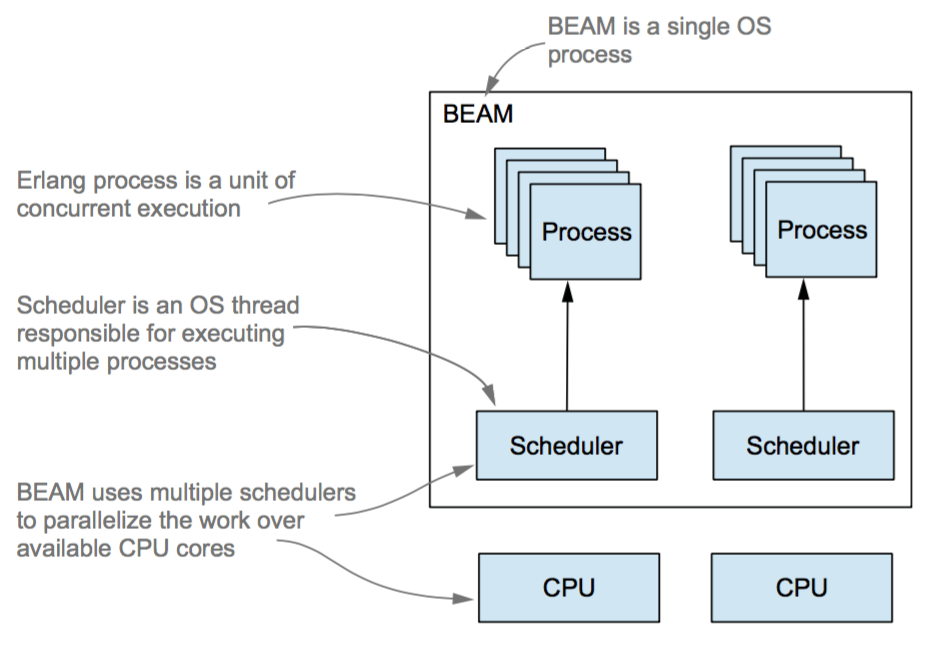
\includegraphics[scale=.5]{beam.png}
  \end{center}
\end{frame}

\begin{frame}
  \frametitle{Server side systems}
  \begin{center}
    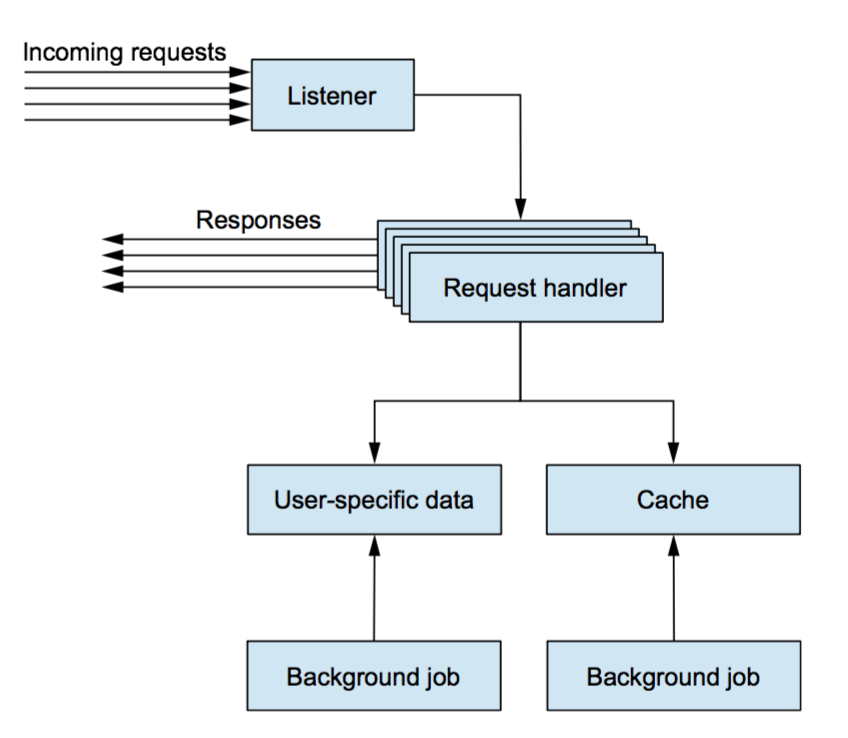
\includegraphics[scale=.5]{otp.png}
  \end{center}
\end{frame}

\begin{frame}
  \frametitle{A modern system}
  \begin{center}
    \begin{tabular}{c|c}
      \hline
      Technical requirements & Server \\ \hline
      HTTP server & Nginx and Phusion Passenger \\
      Request processing & Ruby on Rails \\
      Long-running requests & Java and Go \\
      Server-wide state & Redis \\
      Persistable data & Redis and MongoDB \\
      Background jobs & Cron, Bash scripts, and Ruby \\
      Service crash recovery & Upstart \\
      \hline
    \end{tabular}
  \end{center}
\end{frame}

\begin{frame}
  \frametitle{OTP}
  \begin{center}
    \begin{tabular}{c|c}
      \hline
      Technical requirements & Server \\ \hline
      HTTP server & Erlang \\
      Request processing & Erlang \\
      Long-running requests & Erlang \\
      Server-wide state & Erlang \\
      Persistable data & Erlang \\
      Background jobs & Erlang \\
      Service crash recovery & Erlang \\
      \hline
    \end{tabular}
  \end{center}
\end{frame}

\section[Section]{Elixir basics}

\begin{frame}
  \frametitle{Syntax}
  ``Elixir syntax is like a marriage of DSL
  friendly Ruby and the powerful hygenic macros of Clojure.``
  \linebreak
  \textrm{-- Devin Torres}
\end{frame}

\begin{frame}[fragile]
  \frametitle{The basics you know}
  \begin{lstlisting}
    1 + 1           # => 2
    2 * (3 + 1) / 4 # => 2.0
    1 + 2; 1 + 3    # => 4

    greeting = "Hello World!"
    IO.puts(greeting)
    # => Hello World!
    # => :ok
  \end{lstlisting}
\end{frame}

\begin{frame}[fragile]
  \frametitle{Modules and function, oh my!}
  \begin{lstlisting}
    defmodule Geometry do
      def rectangle_area(a, b) do
        a * b
      end
    end
  \end{lstlisting}
\end{frame}

\begin{frame}[fragile]
  \frametitle{Composing functions}
  \begin{lstlisting}
    def process_xml(model, xml) do
      model
      |> update(xml)
      |> process_changes
      |> persist
    end
  \end{lstlisting}
\end{frame}

\begin{frame}[fragile]
  \frametitle{Function arity}
  \begin{lstlisting}
    defmodule Rectangle do
      def area(a), do: area(a, a)
      def area(a, b), do: a * b
    end
  \end{lstlisting}
\end{frame}

\begin{frame}[fragile]
  \frametitle{Destructuring}
  \begin{lstlisting}
    def do_something({:ok, value}) do
      # use the value here
    end

    def do_something({:warning, value}) do
      # warn user before proceeding
    end

    def do_something({:error, message}) do
      # produce a nice error message to the user
    end
  \end{lstlisting}
\end{frame}

\begin{frame}[fragile]
  \frametitle{Typespec}
  \begin{lstlisting}
    defmodule Circle do
      @pi 3.14159

      @spec area(number) :: number
      def area(r), do: r * r * @pi
        
      @spec circumference(number) :: number
      def circumference(r), do: 2 * r * @pi
    end
  \end{lstlisting}
\end{frame}

\section[Section]{Macros}

\begin{frame}
  \frametitle{Macros}
  \begin{itemize}
  \item code transformation at compile time
  \item code that can change semantics of the input
  \item a lot of elixir functionality is implemented in macros \textsl{e.g. def, unless}
  \item should be used sparingly
  \end{itemize}
\end{frame}

\begin{frame}[fragile]
  \frametitle{Macro expension}
  \begin{columns}
    \column {.5\textwidth}
    \begin{lstlisting}
      unless some_exp do
        block_1
      else
        block_2
      end
    \end{lstlisting}
    \column {.5\textwidth}
    \begin{lstlisting}
      if some_exp do
        block_2
      else
        block_1
      end
    \end{lstlisting}
  \end{columns}
\end{frame}

\begin{frame}[fragile]
  \frametitle{Quoting}
  \begin{lstlisting}
    quote do: sum [1, 2, 3]
    # => { :sum, [], [1, 2, 3] }

    quote do: 1 + 1
    # => { :+,
    #      [context: Elixir, import: Kernal],
    #      [1, 1] }
  \end{lstlisting}
\end{frame}

\begin{frame}[fragile]
  \frametitle{Simple macro}
  \begin{lstlisting}
    defmacro match?(left, right) do
      quote do
        case unquote(right) do
          unquote(left) ->
            true
          _ ->
            false
        end
      end
    end
  \end{lstlisting}
\end{frame}

\begin{frame}[fragile]
  \frametitle{Usine our new macro!}
  \begin{lstlisting}
    list = [{:a,1},{:b,2},{:a,3}]
    # => [a: 1, b: 2, a: 3]

    Enum.filter list, fn (thing) do
      match?({:a, _}, thing)
    end
    # => [a: 1, a: 3]

    Enum.filter list, match?({:a, _}, &1)
    # => [a: 1, a: 3]
  \end{lstlisting}
\end{frame}

\section[Section]{Tooling and Abstractions}
  
\end{document}
